%!TEX root = ../egpaper_final.tex

\section{Approach}

Our pipeline is summarized in Figure \ref{overview-diagram}. We begin with a pair of RGB stereo images. From this image pair and calibration parameters obtained offline, we apply a stereo matching algorithm [See TODO] to get a depthmap of the scene. Using camera instrinsic parameters, we can project this depthmap into 3D space and obtain a point cloud of the environment [See TODO]. We segment locations in the left RGB image that are likely candidates for planar surfaces, and sample corresponding points in the point cloud to obtain an estimate for the parameters of a plane. Finally, we construct a polytope of the object in front of the robot by joining the planar surfaces that we detect. The robot can then use this geometric representation of the terrain to plan its foot trajectory.


\begin{figure}[!h]
\centering
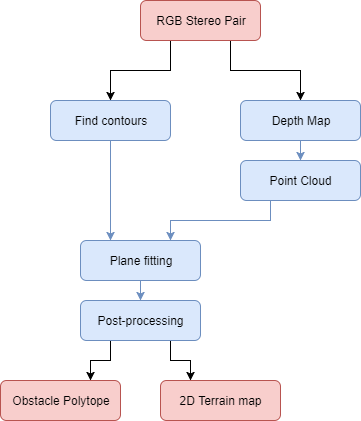
\includegraphics[width=2in]{Sections/Figures/Final-Project-Pipeline.png}
\caption{An overview of our obstacle reconstruction pipeline.}
\label{overview-diagram}
\end{figure}

\subsection{Stereo Matching}

\begin{figure}[!h]
\centering
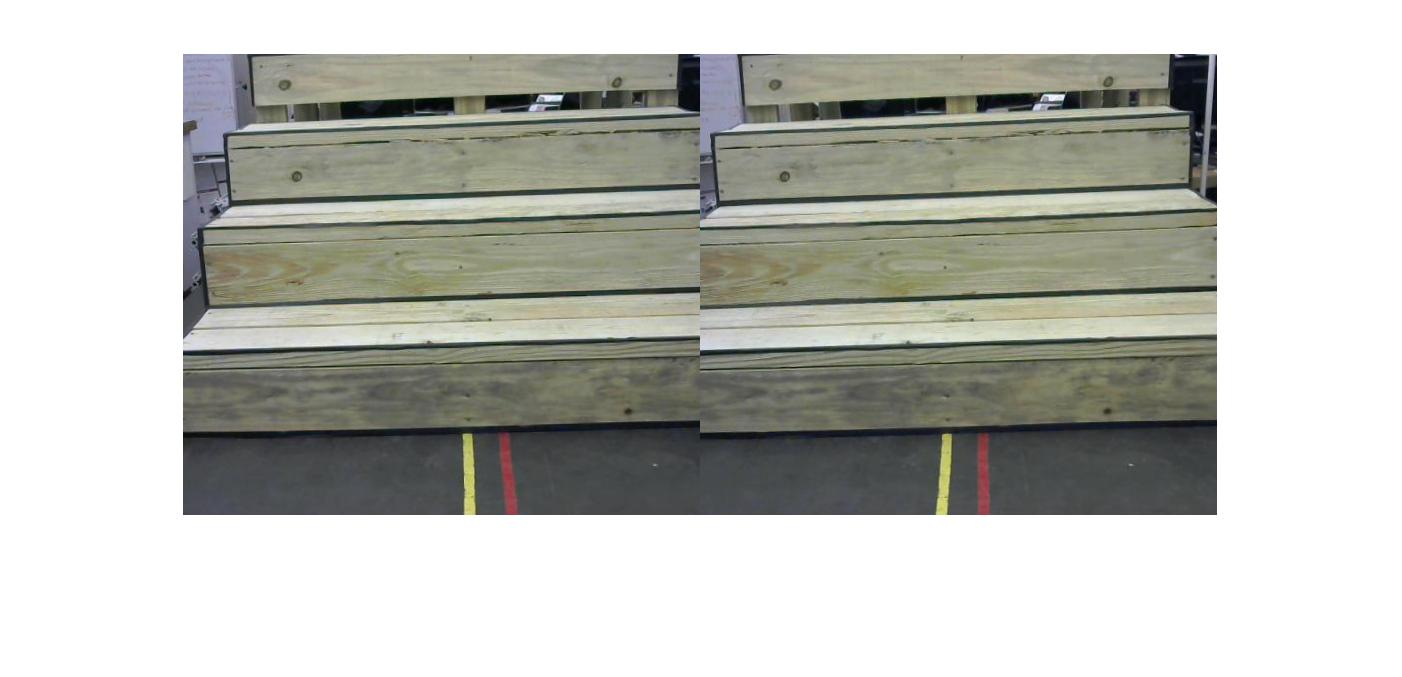
\includegraphics[width=3.3in]{Sections/Figures/example_stereo_pair.jpg}
\caption{An example stereo image pair taken by our camera setup. The two cameras are parallel and have a baseline of approximately 8cm.}
\label{stereo-image-pair}
\end{figure}

\begin{figure}[!h]
\centering
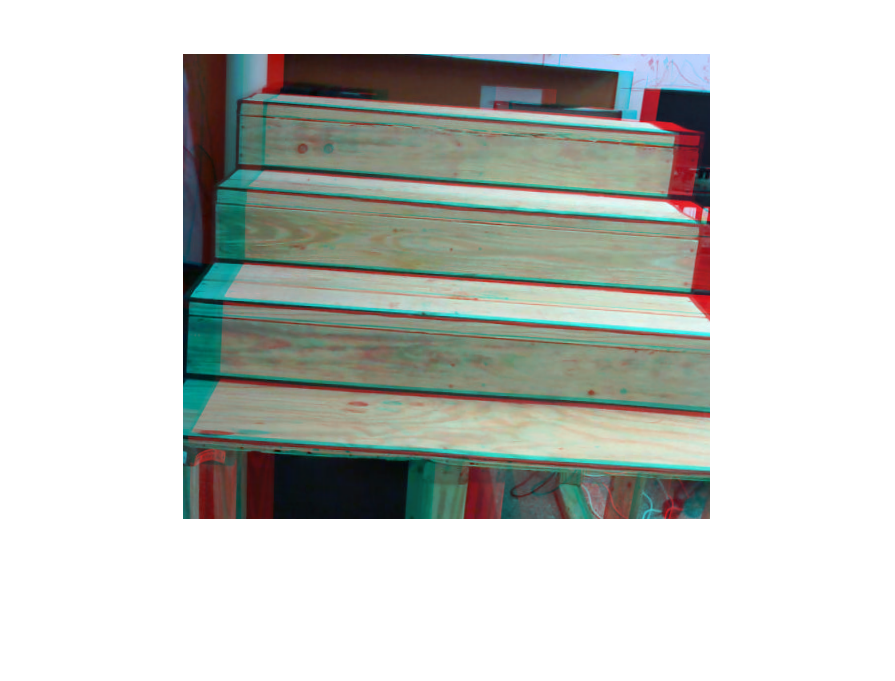
\includegraphics[width=3.3in]{Sections/Figures/stereo_anaglyph.png}
\caption{An example stereo anaglyph.}
\label{stereo-anaglyph}
\end{figure}

\subsection{Point Cloud from Depthmap}

\begin{figure}[!h]
\centering
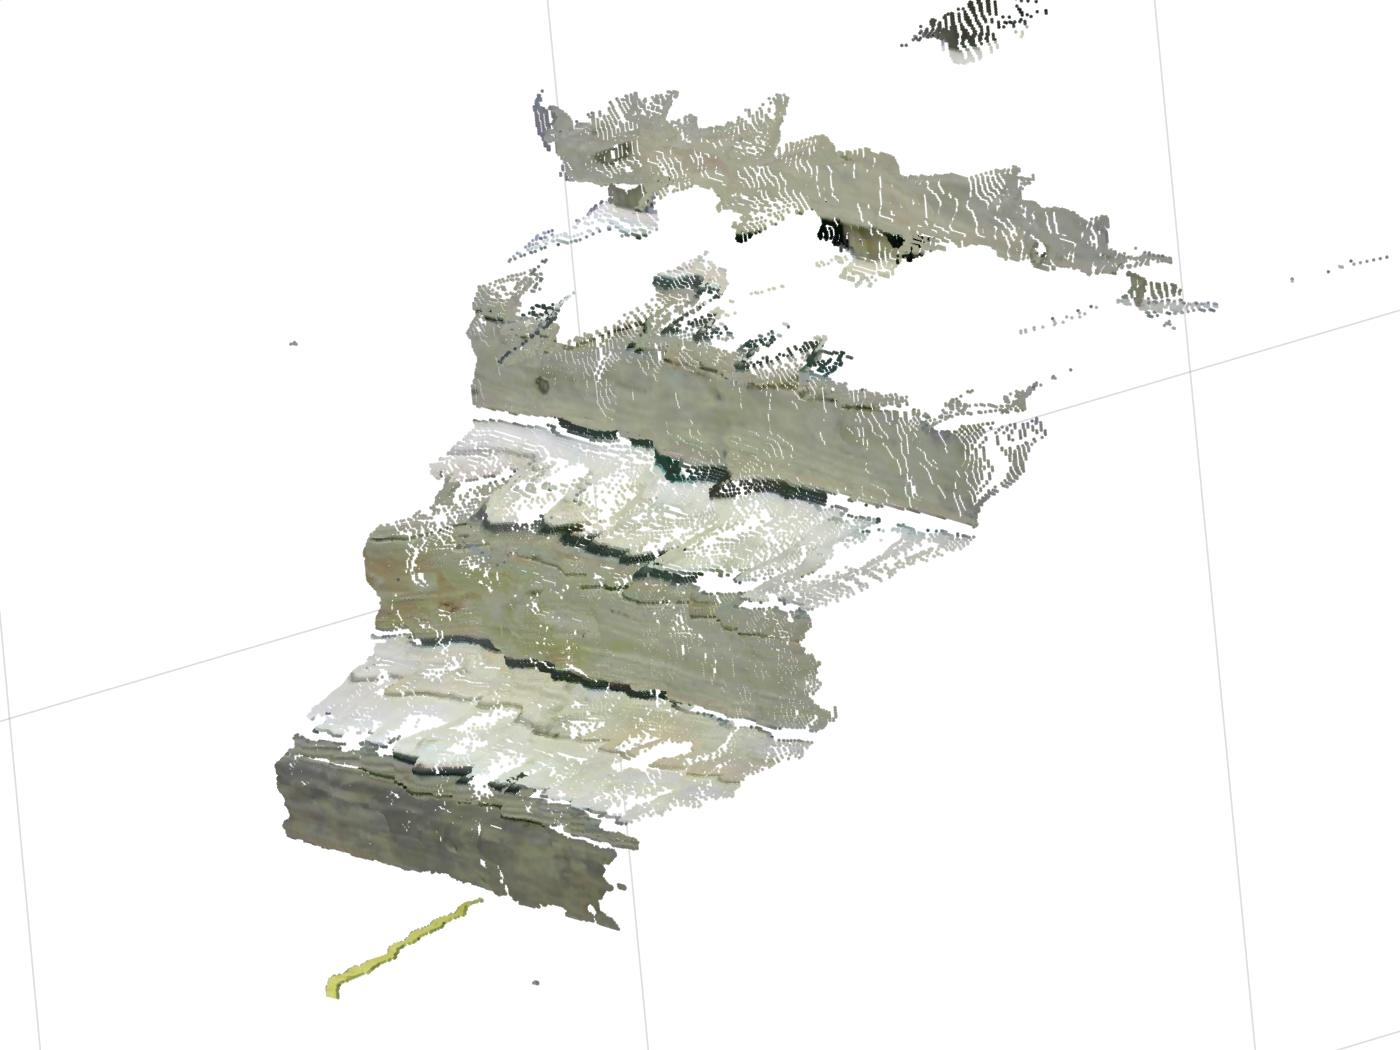
\includegraphics[width=3.3in]{Sections/Figures/example_stairs_pointcloud.jpg}
\caption{A pointcloud representation of the set of stairs in Figure \ref{stereo-image-pair}.}
\label{pointcloud-example}
\end{figure}

\subsection{Polytope Estimation of Objects}

\begin{figure}[!h]
\centering
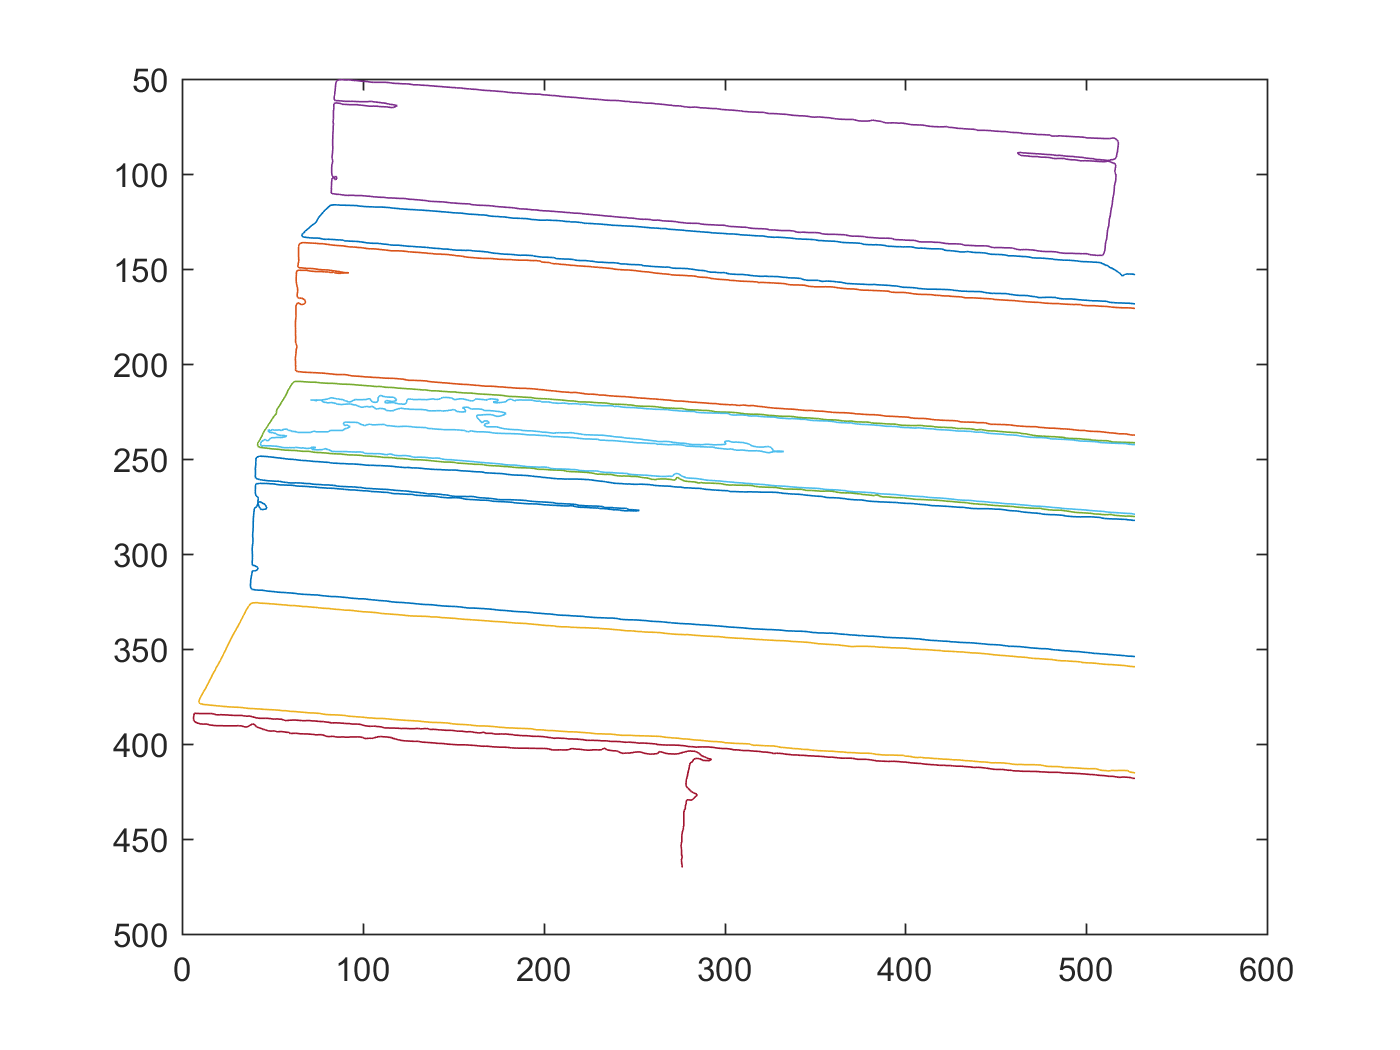
\includegraphics[width=3.3in]{Sections/Figures/good_contour_plot_12-7.png}
\caption{An example contour plot of the stairs in Figure \ref{stereo-anaglyph}. Here we have shown the eight largest contours in the image by area.}
\label{contours-example}
\end{figure}

\begin{figure}[!h]
\centering
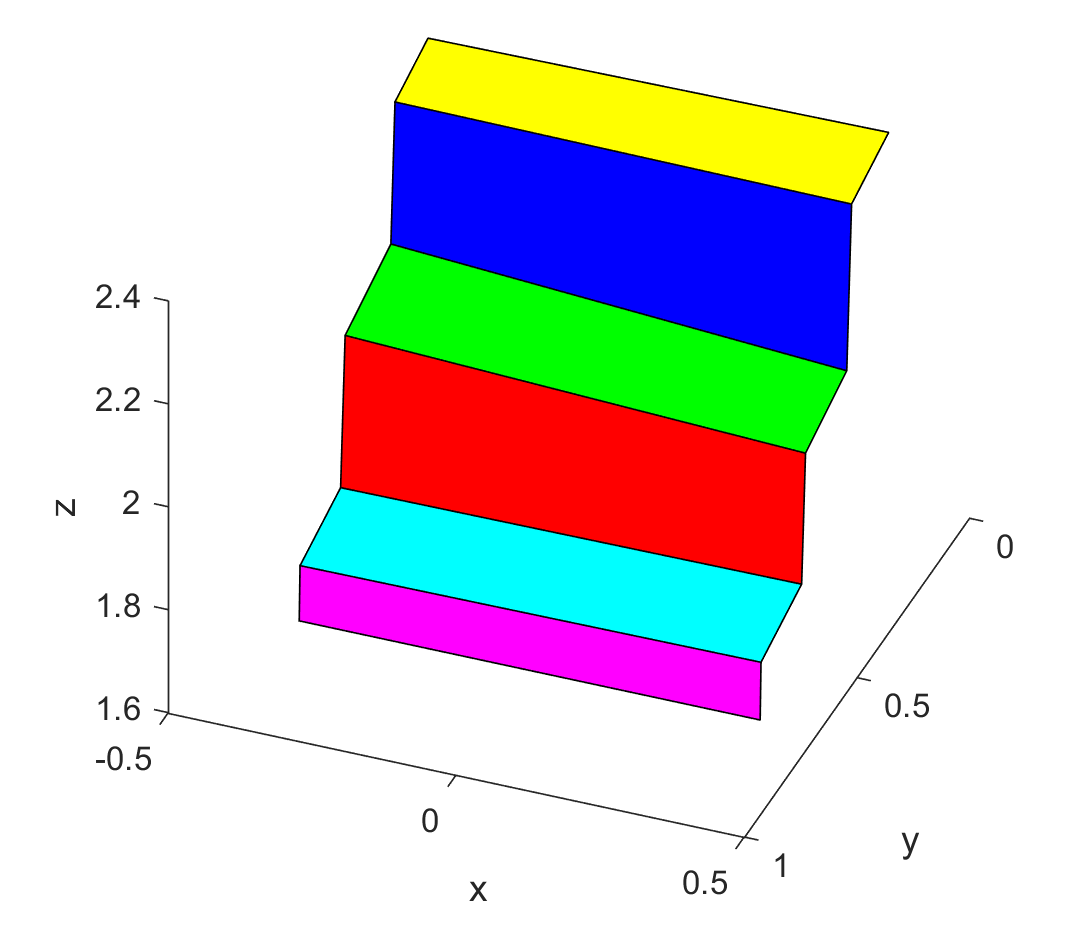
\includegraphics[width=3.3in]{Sections/Figures/polytope_example.png}
\caption{The output of our pipeline when applied to the stereo pair in Figure \ref{stereo-image-pair}. The pink, red, and blue planes correspond to horizontal faces of the stairs. The light-blue, green, and yellow planes are vertical faces.}
\label{polytope-diagonal}
\end{figure}

\begin{figure}[!h]
\centering
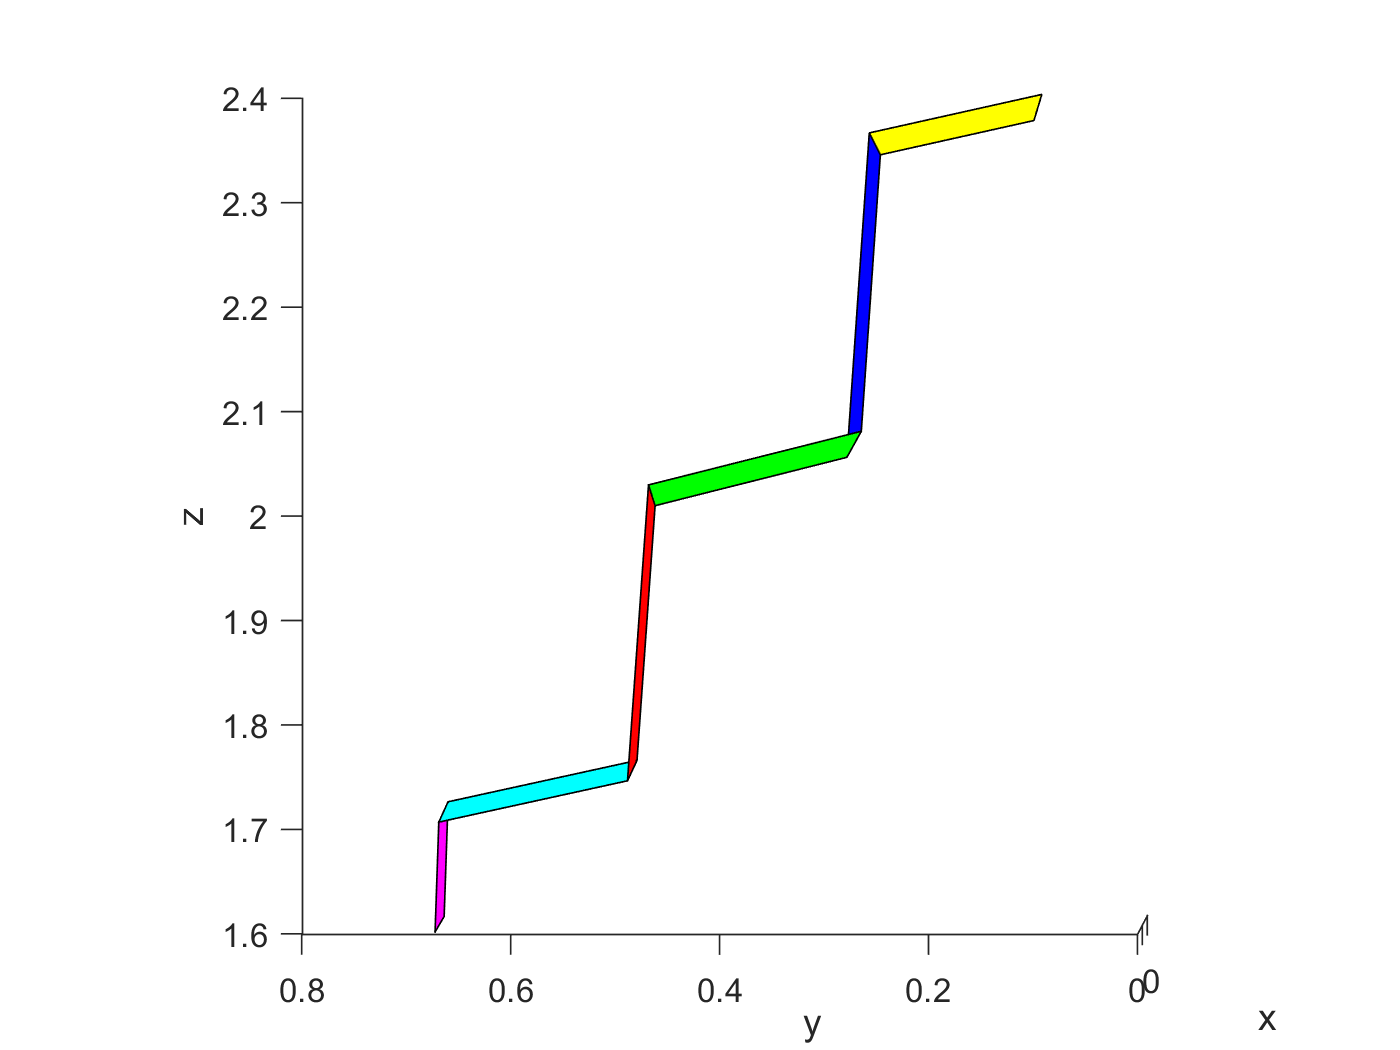
\includegraphics[width=3.3in]{Sections/Figures/polytope_sideview.png}
\caption{The polytope from Figure \ref{polytope-diagonal} viewed from the side. The vertical faces of this polytope (light-blue, green, yellow) are very close to the groundtruth dimension of 20cm. Similarly, the remaining horizontal faces are close to their groundtruth dimension of 31cm. Note that the pink plane is cut off by a bounding box around the polytope, so it does not appear to be the correct size.}
\label{polytope-sideview}
\end{figure}